
\documentclass[11pt,largemargins]{homework}
\usepackage{xcolor}
\usepackage{graphicx}

% TODO: replace these with your information
\newcommand{\hwname}{Elias, Guillermo, Maggie, Sam, Simon, Thomas}
\newcommand{\hwemail}{}
\newcommand{\hwtype}{Big Pset}
\newcommand{\hwnum}{}
\newcommand{\hwclass}{AST 301}
\newcommand{\hwlecture}{}
\newcommand{\hwsection}{}

\begin{document}
\maketitle

%====================== Question 1 ===========================
\question
In frame $O$, a meter stick lies parallel to the $x$ axis and moves at velocity $V \mathbf{e}_y$.  Frame $\bar{O}$ is boosted relative to $O$ at velocity $\beta \mathbf{e}_x$ but not rotated, i.e., the spatial axes $\bar{x}\bar{y}\bar{z}$ lie parallel to $xyz$.  Show that in $\bar{O}$, the meter stick makes a nonzero angle $\theta$ with respect to the $\bar{x}$ axis, and derive an expression for $\theta$ in terms of $V$ and $\beta$. 

We use the relativistic velocity formulae, referencing Hartle (4.28), which assumes that as in our problem, the barred or primed frame is moving with some velocity in the $x$-drection.  Namely
\begin{subequations}
\begin{align}
V^{\bar{x}} &= \frac{V^{x} - v}{1 - v V^{x} / c^2}, \\
V^{\bar{y}} &= \frac{V^{y}}{1 - v V^{x} / c^2} \sqrt{1 - v^2 / c^2}.
\end{align}
\end{subequations}
Setting $c = 1$ and realizing $V^{x} = 0$, $V^{y} = V$, and $v = \beta$, we have
\begin{subequations}
\begin{align}
V^{\bar{x}} &= -\beta, \\
V^{\bar{y}} &= V \sqrt{1 - \beta^2}.
\end{align}
\end{subequations}
Recall that $\theta = \mathrm{arctan}(y / x)$, so 
\begin{equation}
\theta = \mathrm{arctan}(\frac{-V \sqrt{1 - \beta^2}}{\beta})
\end{equation}

%===================== Question 2 ===============================
\question
Observer $O$ constructs a clock in which a photon bounces back and forth along the $x$ axis at $x = 0$ and $x = L$. $O$ moves at speed $(4/5)c$ relative to $\bar{O}$ along the $x \bar{x}$ axis. 
\begin{alphaparts}

\questionpart
What is the round trip time between the two mirrors in frames $O$ and $\bar{O}$?
In frame $O$ the round trip time is simply the total distance $2L$ divided by $c$, i.e
\begin{equation}
\tau = \frac{2L}{c}
\end{equation}
To find the round trip time we use Hartle (4.15), which states
\begin{equation}
d\tau = d\bar{t} \sqrt{1 - V^2 / c^2}.
\end{equation}
For us, $d\tau = 2L/c$, so
\begin{subequations}
\begin{align*}
\frac{2L}{c} &= d\bar{t} \sqrt{1 - V^2 / c^2}, \\
d\bar{t} &= \frac{2L/c}{\sqrt{1 - V^2 / c^2}}, \\
d\bar{t} &= \frac{5}{3} \frac{2L}{c},
\end{align*}
\end{subequations}
Thus, the round trip time in $\bar{O}$ is
\begin{equation}
\bar{t} = \frac{10L}{c}
\end{equation}

\questionpart
What is the separation between the mirrors in $\bar{O}$?
Recall that 
\begin{equation}
\bar{L} = \frac{1}{\gamma} L_{0},
\end{equation}
where $L_{0}$ is the length in the rest frame.
Then
\begin{equation}
\bar{L} = \frac{3}{5} L
\end{equation}

\questionpart
The energy of the photon is $E$ in $O$.  What energy does $\bar{O}$ measure for the photon while it travels from $x = 0$ to $x = L$, and what energy does she measure while it travels from $x = L$ to $x = 0$?  (The mirrors are too massive to recoil appreciably.)

\begin{subequations}
\begin{align*}
E_{\mathrm{left}} &= \gamma \frac{E}{c} (1 + \beta) \\
&= \frac{1}{\sqrt{1 - (4/5)^2}} \frac{E}{c} (1 + 4/5) \\
&= \frac{3E}{c} \\ \\
E_{\mathrm{right}} &= \gamma \frac{E}{c} (1 - \beta) \\
&= \frac{1}{\sqrt{1 - (4/5)^2}} \frac{E}{c} (1 - 4/5) \\ 
&= \frac{E}{3c}
\end{align*}
\end{subequations}

\questionpart
If there are $N$ such photons distributed uniformly between the mirrors, all moving parallel to the $x$ axis, and with equal numbers moving in each direction as seen in $O$; and if the surface of each mirror is $A$, what are the components of the energy-momentum tensor due to these photons in frames $O$ and $\bar{O}$?

The energy momentum tensor $T$ is a rank 2 tensor, which means it can be represented by an ordinary matrix.  We have one spatial dimension and the time dimension, so it is represented by a $2 \times 2$ matrix.  Our strategy will be to find the components of $T$ in the frame $O$, and then use the Lorentz transform to find the components in $\bar{O}$. Then, in frame $O$: 

$T^{00}$ is the energy density, or the energy/volume.  So 
$$T^{00} = \frac{NE}{AL},$$ where E is the energy of each photon.  The $T^{10} = T^{01}$ components are the momentum density, which are zero.  The remaining component $T^{11}$ is the force per area in the x-direction.  (A full description of the energy-momentum tensor is given in the solution to problem 6.) Then,
\begin{subequations}
\begin{align*}
T^{11} &= \frac{N}{2AL} \frac{E}{c} c + \frac{N}{2AL} \frac{-E}{c} (-c) \\
&= \frac{NE}{AL}
\end{align*}
\end{subequations}
Therefore, in $O$:

\begin{equation}
T = \frac{NE}{AL} \begin{pmatrix} 1 & 0 \\ 0 & 1 \end{pmatrix}
\end{equation}

To find the components of $T$ in $\bar{O}$, we perform a Lorentz transform.  Because we have two components for $T$, we have to do a matrix multiplication for each component.  The form of these matrix multiplications is
\begin{equation}
T^{\bar{\mu}\bar{\nu}} = \big[ \Lambda_{\nu}^{\bar{\nu}} \big]^{\top} T^{\mu \nu} \big[ \Lambda_{\mu}^{\bar{\mu}} \big]
\end{equation}
Therefore, in $\bar{O}$

\begin{equation*}
T^{\bar{\mu} \bar{\nu}} = \frac{NE}{AL} \begin{pmatrix} \gamma & \gamma \beta \\ \gamma \beta & \gamma \end{pmatrix} \begin{pmatrix} 1 & 0 \\ 0 & 1 \end{pmatrix} \begin{pmatrix} \gamma & \gamma \beta \\ \gamma \beta & \gamma \end{pmatrix} 
\end{equation*}

\begin{equation}
T^{\bar{\mu} \bar{\nu}} = \frac{NE}{AL} \begin{pmatrix} \gamma^2 + \gamma^2 \beta^2 & 2 \gamma^2 \beta \\ 2 \gamma^2 \beta & \gamma^2 \beta^2 + \gamma^2 \end{pmatrix}
\end{equation}
\end{alphaparts}

%=============== Question 3 ===================
\question An optical fiber of index of refraction $n > 1$ is bent into a circular ring of radius $r$ (much larger than the diameter of the fiber itself).  As seen from an inertial frame $O$, the ring rotates counterclockwise around its center at angular velocity $\Omega < c/r;$ the center of the ring is at rest in $O$.

\begin{alphaparts}
\questionpart
Calculate in frame $O$ the travel time of a light beam going once around the ring counterclockwise and returning to the same angular position as seen in $O$.  Let this be called $t_{+}$. 

In the stationary (lab) frame, the speed of light becomes $c/n$, so 
\begin{equation}
t_{+} = \frac{2 \pi r n}{c}
\end{equation}

\questionpart 
Now calculate the time $\bar{t}_{+}$ in the local rest frame of a station along the fiber.

We now have to do a Lorentz transform, realizing that
$$\bar{t}_{+} = \gamma (t_{+} - vx),$$
where $v = \Omega r$ and $x = 2 \pi r$. Therefore,
\begin{equation}
\bar{t}_{+} = \gamma 2 \pi r \big(\frac{n}{c} - \Omega r\big)
\end{equation}
where $\gamma = 1/\sqrt{1 - \Omega^2 r^2 / c^2}$.

\questionpart
Similarly calculate the corresponding times $t_{-}$ and $\bar{t}_{-}$ for clockwise beams, and thereby obtain the difference $\Delta \bar{t}$ in terms of $\Omega$ and $r$. 

It is clear that $t_{-}  = t_{+}$, because the direction of rotation already did not matter for $t_{+}$.  For $\bar{t}_{-}$, simply consider that it is the same as changing the sign of the velocity in the Lorentz transform, i.e.,
$
\bar{t}_{-} = \gamma (t_{-} + vx) = \gamma 2 \pi r \big(\frac{n}{c} + \Omega r \big)
$
Then to find $\Delta \bar{t}$, we just take the difference, and find
\begin{equation}
\Delta \bar{t} = \gamma 4 \pi \Omega r^2 .
\end{equation}
\end{alphaparts}	

%================== Question 4 =================
\question
Approximately 19 neutrinos were detected from supernova 1987A in the Large Magellanic Cloud.  The neutrinos arrived over a span of about 15 seconds with energies ranging from roughly 10 to 40 MeV.  Given that the distance to the LMC is approximately 50 kpc $\approx 5 \times 10^12$ lt sec, and assuming that the supernova did not conspire to emit the lower-energy neutrinos before the higher-energy ones, estimate a rough upper bound to the neutrino rest mass.

Our strategy will be to solve for the velocity of the neutrino in terms of its mass and energy, and then compute a bound for the mass given the difference in velocities based on the different energies.
The energy of a neutrino (or any particle) is given by (Hartle 5.49)
\begin{subequations}
\begin{align}
E &= (m^2 + \bar{p}^2)^{1/2} \\
\nonumber &= (m^2 + (m \gamma \bar{v})^2)^{1/2} \\
\nonumber &= m(1 + \frac{v^2}{1-v^2})^{1/2} 
\end{align}
\end{subequations}
Then we solve explicitly for v.
\begin{subequations}
\begin{align*}
E^2 &= m^2(1 + \frac{v^2}{1-v^2}) \\
\frac{E^2}{m^2} - 1 &= \frac{v^2}{1 - v^2} \\
v &= \sqrt{\frac{\frac{E^2}{m^2} - 1}{\frac{E^2}{m^2}}} \\
v &= \sqrt{1 - \frac{m^2}{E^2}}
\end{align*}
\end{subequations}
The time it takes for a neutrino to arrive is $D/v$, so the difference is $D/v_{1} - D/v_{2} = 15 \mathrm{s}$.  With proper units, this gives us

\begin{equation}
15 \mathrm{s} = 50 \mathrm{kpc} \Bigg[ \frac{1}{\sqrt{c^2 - \frac{m^2 c^6}{E_{2}^2}}} - \frac{1}{\sqrt{{c^2 - \frac{m^2 c^6}{E_{1}^2}}}} \Bigg]
\end{equation}

Dividing through by 50 kpc, factoring out a c from the denominator and multiplying through by c, and cleverly factoring the denominator, we find:

\begin{equation}
1.46 \times 10^{-10} = \frac{1}{\sqrt{1 - \frac{mc^2}{E_2}} \sqrt{1 + \frac{mc^2}{E_2}}} - \frac{1}{\sqrt{1 - \frac{mc^2}{E_1}} \sqrt{1 + \frac{mc^2}{E_1}}}
\end{equation}

Noting that $E_2 = 10$ MeV, $E_1 = 40$ MeV, and $mc^2 = M_{\mathrm{bound}}$, we find
$M_{\mathrm{bound}} / E_{2} = 1.76 \times 10^{-5}$ Therefore, $M_{\mathrm{bound}} = 17.6$ meV. 

\setcounter{questionCounter}{5}

%==================== Question 6 =================================
\question
Consider an idealized spherical dust grain of radius $a_g$ and mass density $\rho_g$ that absorbs optical light with cross section $\pi a^2$ and re-radiates an equivalent energy isotropically in its rest frame.  Let such a grain be in a circular orbit about the Sun (mass $M_{\odot} = 2 \times 10^{33} \mbox{ g}$, luminosity $L_{\odot} = 4 \times 10^{33} \mbox{ erg} \mbox{ s}^-1$) at an orbital radius equal to that of the Earth: $1 \mbox{ AU} = 1.5 \times 10^{13} \mbox{ cm}.$ 

\begin{alphaparts}
\questionpart
What is the stress-energy tensor of the solar radiation in the local rest frame of the grain? You may neglect the angular size of the sun and assume that the photons move perfectly radially.  

We first want to find $T^{\bar{\mu}\bar{\nu}}$ in the local frame at rest with respect to the sun, and then boost along the grains orbital motion, $30 \mbox{ km} \mbox{ s}^{-1}$.  Let's take a moment, however, to make sure we understand the stress-energy (aka energy-momentum) tensor.  It's a symmetric rank two tensor which can be represented by an $n \times n$ matrix, where $n$ is the number of dimensions: in this case, $1 + 3$. $T^{00}$ is the energy density.  If $p$ is the 4-momentum, $T^{00} = \Delta p^{t} / \Delta V$, where $V$ is the volume.  The $T^{0i}$ row is the energy flux, and it equals the $T^{i0}$ column, which is the momentum density, $\Delta p^{i} /\Delta V$. The $T^{ij}$ components are the normal stress tensor, the force exerted in the $i$ direction over the area of the surface normal to the $j$ direction.  The diagonal components are therefore the pressure.  

For the grain, $T^{\bar{0}\bar{0}} = \rho / V = 3\rho_{g} / 4 \pi a^3$. All the pressure exerted on the dust grain by the Sun will be in the $r$ direction, so we can just find $T^{\bar{r}\bar{r}}$. It's the force on the grain over the area of the grain, so it ends up canceling to the flux on the grain: $L/4 \pi r^2$. It so happens that this is the same for $T^{\bar{0}\bar{r}}$ and $T^{\bar{r}\bar{0}}$.  Now let's apply the Lorentz boost in the $\theta$ direction.  Let's note that 
$$\Lambda_{\bar{\mu}}^{\mu} = \begin{pmatrix} \gamma & 0 & -v\gamma & 0 \\ 0 & 1 & 0 & 0 \\ -v \gamma & 0 & \gamma & 0 \\ 0 & 0 & 0 & 1 \end{pmatrix}. $$

Now it's a matter of solving for each of the components of the stress-energy tensor in the boosted frame.  We could do the matrix multiplication, but we can also solve it componentwise.  Since we used matrix multiplication in problem 2, lets use the components here, noting that 
\begin{equation}
T^{\mu \nu} = \Lambda_{\bar{\mu}}^{\mu} \Lambda_{\bar{\nu}}^{\nu} T^{\bar{\mu} \bar{\nu}}.
\end{equation}  Although this looks a lot like equation 13, it's not quite the same.  This is because it actually is an expression for each component rather than the matrix form of the equation.  This is a subtle difference and it is important to stay on top of it.  Now we can compute the entries of $T^{\mu \nu}$, taking care to observe that it is a symmetric tensor.
\begin{subequations}
\begin{align*}
T^{00} &= \Lambda_{\bar{0}}^{0} \Lambda_{\bar{0}}^{0} T^{\bar{0}\bar{0}} = \gamma^2 \frac{3 \rho}{4 \pi a^3} \\ \\
T^{rr} &= \Lambda_{\bar{r}}^{r} \Lambda_{\bar{r}}^{r} T^{\bar{r}\bar{r}} = \frac{L}{4 \pi r^2} \\ \\
T^{0r} &= \Lambda_{\bar{0}}^{0} \Lambda_{\bar{r}}^{r} T^{\bar{0}\bar{r}} = \frac{L}{4 \pi r^2} \gamma = T^{r0} \\ \\ 
T^{\theta \theta} &= \Lambda_{\bar{0}}^{\theta} \Lambda_{\bar{0}}^{\theta} T^{\bar{0}\bar{0}} = \frac{3 \rho}{4 \pi a^3} v^2 \gamma^2. \\ \\
T^{\theta 0} &= \Lambda_{\bar{0}}^{\theta} \Lambda_{\bar{0}}^{0} T^{\bar{0}\bar{0}} = -\frac{3 \rho}{4 \pi a^3} v \gamma = T^{0 \theta} \\ \\
T^{r \theta} &= \Lambda_{\bar{r}}^{r} \Lambda_{\bar{0}}^{\theta} T^{\bar{r}\bar{0}} = - \frac{L}{4 \pi r^2} v \gamma = T^{\theta r}
\end{align*}
\end{subequations}

\questionpart 
Find expressions for the radial and azimuthal forces on the grain due to solar radiation.  (We skip the trivial evaluation step.) 

This is what the stress tensor is for!  We can just say that $F_{r} = T^{rr} \pi a^2.$ and $F_{\theta} = T^{\theta \theta} \pi a^2$. Therefore,
\begin{subequations}
\begin{align}
F_r &= \frac{L a^2}{4 r^2} \\
F_{\theta} &= \frac{3 \rho}{4 a} v^2 \gamma^2
\end{align}
\end{subequations}
\end{alphaparts}

%===================== Question 7 ==================

\question
A two-dimensional spacetime has metric
$$ ds^2 = -xdv^2 + 2dvdx. $$

\begin{alphaparts}

\questionpart
Write down the equations and constants of motion for timelike geodesics in the coordinates $(x, v)$.  Solve for $x(\tau)$ and $v(\tau).$ 

For a question like this our plan of attack is to use the geodesic equation.  We should expect to find one constant of motion from the geodesic equation, and in this case we should expect to find another from the metric.  For a timelike particle, the geodesic equation is 

\begin{equation}
\frac{d}{d\lambda} \Bigg(g_{\alpha \nu} \frac{dx^{\nu}}{d\lambda} \Bigg) - \frac{1}{2} g_{\mu \nu, \alpha} \frac{dx^{\mu}}{d\lambda} \frac{dx^{\nu}}{d\lambda} = 0
\end{equation}

Let's note from the metric that $g_{vv} = -x$; $g_{xx} = 0$; and $g_{vx} = g_{xv} = 1$. 
We also see that none of the metric coefficients depend on $v$.  Therefore, if $\alpha = v$, $g_{\mu \nu, \alpha} = 0$. So we should expect a constant of motion for that.  Indeed, we find 
$$
g_{vv} \frac{dv}{d\lambda} + g_{vx} \frac{dx}{d\lambda} = k
$$
Where $k$ is a constant.  Explicitly,
$$
-x \frac{dv}{d\lambda} + \frac{dx}{d\lambda} = k.
$$

Our second constant of motion comes from the fact that the product of the 4-velocity with itself is always $-1$.

$$
\bigg(\frac{ds}{d\lambda}\bigg)^2 = -1.
$$
Therefore
$$
-x \bigg(\frac{dv}{d\lambda}\bigg)^2 + 2 \frac{dv}{d\lambda} \frac{dx}{d\lambda} = -1.
$$

Our goal now is to take our constants of motion and find a quadrature which we can integrate in order to get $x(\tau)$ and $v(\tau)$. We start by using our first constant of motion to solve for $dv/d\lambda$ and then find a quadrature for $x$.

\begin{subequations}
\begin{align*}
\frac{dv}{d\lambda} &= \frac{\frac{dx - k}{d\lambda}}{x} \\ \\
\frac{\frac{dx}{d\lambda}- k}{x} \bigg(-\big(\frac{dx}{d\lambda} - k\big) + 2\big(\frac{dx}{d\lambda}\big) \bigg) &= -1 \\ \\
\text{Notice that we can factor this.  Doing so, we find} \\ \\ 
\big(\frac{dx}{d\lambda} + k\big) \big(\frac{dx}{d\lambda} - k \big) + x &= 0 \\ \\
\big(\frac{dx}{d\lambda}\big)^2 &= k^2 - x^2 \\ \\
\frac{dx}{\sqrt{k^2 - x}} &= \pm dt \\ \\
\text{Now we can integrate both sides of this equation, which yields} \\ \\ 
2 \sqrt{k^2 - x} &= \pm (\tau - \tau_{0}) \\ \\
\text{Solving for x, we find} \\
x(\tau) &= k^2 - \frac{(\tau - \tau_0)^2}{4}
\end{align*}
\end{subequations}

Now we can plug our answer for $x$ back into our answer for $dv / d\lambda$ and solve for $v(\tau)$. Note that $\lambda = \tau$ (I guess?  Lol.) Doing so, we find

\begin{subequations}
\begin{align*}
\frac{dv}{d\tau} &= \frac{\frac{(\tau - \tau_0)}{2} - k}{k^2 - \frac{(\tau - \tau_0)^2}{4}} \\ \\ 
v(\tau) &= -2 \ln (2k + \tau - \tau_0)
\end{align*}
\end{subequations}

\questionpart
$v$ is obviously a null coordinate.  Find a second null coordinate -- call it $u$ -- and express $x$ as a function of $(u, v)$.

A coordinate $a$ is null if setting $da = 0$ implies $ds^2 = 0$. So we want to find a function $u(x,v)$ so that we can set $du = 0$ and recover $ds^2 = 0$.  Let's factor a $-x$ out of our metric.  Doing so, we find
\begin{subequations}
\begin{align*}
ds^2 &= x \cdot (2 dv dx/x - dv^2) \\ 
&= x dv \cdot (2 dx/x - dv^2) \\ 
&= x dv \cdot d(2\ln(x) - v)
\end{align*}
\end{subequations}
Therefore,
$$
u = 2 \ln(x) - v
$$
and
$$ x = e^{(u+v)/2} $$

\questionpart
Find coordinates $X$, $T$ as functions of $u$, $v$ such that $ds^2 - -dT^2 + dX^2$, hence showing that the metric describes flat space.

Let's try and get our function $x(u,v)$ out of the metric.  To do so, we introduce variables $U$ and $V$.  $dU = e^{u/2} du$ and $dV = e^{v/2} dv$.  Then $U = 2e^{u/2}$ and $V = 2e^{v/2}.$  More importantly, $ds^2 = -dUdV$. \\ 

Let's set $U = T + X$ and $V = T - X$.  Then note that $dU = dT + dX$ and $dV = dT - dX$.  Therefore, 
$$ ds^2 = - dU dV = (-dT^2 + dX^2) $$

Which describes flat space.  The space may not have looked flat before, but that was an artifact of the coordinates.

\end{alphaparts}

%====================== Question 8 ================= %

\question
Averaged over orbits about the Sun, how much slower or faster does a perfect atomic clock on the surface of Mars run compared to one on the surface of Earth?  For the purpose of this problem, take the mass, radius, and orbital semi-major axis of the Earth to be $M_E \approx 6 \times 10^{27} \mbox{ g}$, $R_E \approx 6.4 \times 10^8 \mbox{ cm}$, and $a_E = 1.5 \times 10^{15} \mbox{ cm}$; and the corresponding values for mars to be $M_M \approx 0.11 M_E$, $R_M \approx 0.53R_E$, and $a_M \approx 1.52a_E$. 

This is a principle of equivalence question.  The clocks will run at different speeds because the gravitational potential from the Sun is different because of their differing radii.  There is also an SR redshift effect because the two planets orbit at different velocities.  Then we can write the principle of equivalence.

\begin{equation}
d\tau^2 = (1 + \frac{2 \Phi}{c^2}) dt^2
\end{equation}
When $\Phi \ll c^2$, we can approximate the square root with a taylor expansion.
\begin{equation}
d\tau \approx (1 + \frac{\Phi}{c^2}) dt
\end{equation}
Incorporating the SR redshift effect, we get:
\begin{equation}
d\tau \approx (1 + \frac{\Phi - v^2/2}{c^2}) dt
\end{equation}

Now we just compare $d\tau_E$ and $d\tau_M$, using (from Kepler's third law or centripetal motion) that $v^2 = GM_{\odot} / a$. Therefore, 
$$
\frac{d\tau_M}{d\tau_E} = \frac{c^2 - \frac{G(0.11)M_E}{(0.53)R_E} - \frac{GM_{\odot}}{2(1.52)a_E}}{c^2 - \frac{GM_E}{R_E} - \frac{GM_{\odot}}{2(a_E}}
$$

Which evaluates to $1 + 5.64 \times 10^{-10}$.

\color{red}
We skip questions 9 and 10 because they will not appear on this year's exam.
\color{black} 
\setcounter{questionCounter}{10}

%===================== Question 11 ================= %
\question
Supermassive black holes reside in the center of most galaxies.  Every $10^4$ yr, typically a star approaches the black hole on a marginally bound, extremely eccentric orbit, with a pericenter $(r_p)$ small enough that the star is \textit{tidally disrupted} if the $\hat{r}\hat{r}$ component of the tidal field is $>GM_{*}/R_{*}^{3}$ where $M_*$ and $R_*$ are the mass and radius of the star.
\begin{alphaparts}
\questionpart
Estimate the maximum $r_p$ for tidal disruption of the Sun in terms of $M_{\mathrm{bh}}$.  $M_{\odot} \approx 2 x 10^{33} \mathrm{g}$, $R_{\odot} \approx 7 x 10^{10} \mathrm{cm}$

Outside a spherical mass of $M_{\mathrm{bh}}$,
\begin{equation}
a_{\hat{r}\hat{r}} = \frac{2M_{\mathrm{bh}}}{r_{p}^{3}},
\end{equation}
according to Hartle (21.8). ($G = 1$ units).  The limit we are concerned with is $a_{\hat{r}\hat{r}} > GM_{*}/R_{*}^{3}$, so we set 
\begin{equation}
\frac{2M_{\mathrm{bh}}}{r_{p}^{3}} = \frac{G M_{*}}{R_{*}^{3}},
\end{equation} 
and solve for $r_{p}$, which yields
\begin{equation}
r_{p} = \bigg(\frac{2 M_\mathrm{bh}}{M_{\odot}} \bigg) ^ {1/3} R_{\odot}
\end{equation}

\questionpart
Just as disrupted/evaporated comets make meteor streams, the debris of a disrupted
star will spread out along the star?s original orbit. However, this leads to
observable consequences only if that orbit does not plunge into the black hole. Estimate the maximum black-hole mass for which a sunlike star can be disrupted on a
non-plunging, marginally-bound orbit.

Our limit for the Innermost Stable Circular Orbit (ISCO) is given by 

\begin{equation}
r_{c} = 6M_{\mathrm{bh}}
\end{equation}
in $G = 1$ units.  (Hartle 9.43 and derived in the lecture 12 slides).  Note that whenever we redimensionalize from mass to radius we simply multiply the mass by a factor of $G/c^2$.  (You can check these units!)

In order to disrupt the star in the non-plunging orbit, we must have $r_{c} > r_{p}$, so to investigate the limiting behavior, we simply set $r_{c} = r_{p}$.  Then we have

\begin{subequations}
\begin{align}
\frac{6 G M_\mathrm{bh}}{c^2} &= \bigg(\frac{2 M_\mathrm{bh}}{M_{\odot}} \bigg) ^ {1/3} R_{\odot} \\
\frac{6G}{2^{1/3}} \frac{M_{\mathrm{bh}}^{2/3}}{c^2} &= R_{\odot} M_{\odot}^{-1/3} \\
M_{\mathrm{bh}} &= \frac{c^3 \sqrt{2}}{6 G^{3/2}} R_{\odot}^{3/2} M_{\odot}^{-1/2}
\end{align}
\end{subequations}
Which we can evaluate for $M_{\mathrm{bh}}$.  Wolfram says it is on the order of $7 x 10^{7} M_{\odot}$.  

\questionpart

Assuming $r_p \gg M$, estimate the radius $r_i \gg r_p$ at which the outgoing part of the orbit intersects the incoming part.  You may use the following approximation for the change in periapse angle per period of a nearly keplerian ($r_p \gg M$) orbit of semi-major axis $a$ and eccentricity $\epsilon:$

\begin{equation}
\delta \phi_{p} \approx \frac{6 \pi M}{a(1 - \epsilon^2)}
\end{equation}

and recall $r_{p} = a(1 - \epsilon)$ and $r(\phi) = a(1 - \epsilon^2) / [1 + \epsilon \cos{(\phi - \phi_{p}})]$.

It's a little tricky to visualize what is going on in this problem, so we've included a figure.  $r_i$ is the intersection between the two ellipses formed here. 
\begin{figure}[h]
\centering
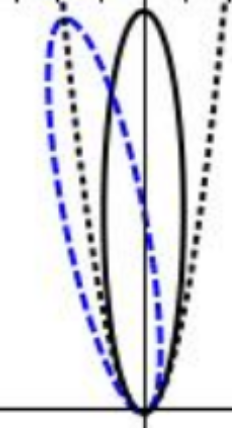
\includegraphics[scale=0.6]{orbits}
\caption{$r_{i}$ is the intersection of the two ellipses.}
\end{figure}

Let's be clear about what this means. The two ellipses are both defined by the equation $r(\phi)$.  The only difference between the two is the argument of the periapsis, $\phi_{p}$.  In order for the two ellipses to intersect, we require:

\begin{equation}
\frac{a(1 - \epsilon^2)}{1 + \epsilon \cos(\phi - \phi_{p})} = \frac{a(1 - \epsilon^2)}{1+\epsilon \cos(\phi - \phi_{p} - \delta \phi_{p})}
\end{equation}

But all this means is that $\cos(\phi - \phi_{p}) - \cos(\phi - \phi_{p} - \delta \phi_{p})$. This seems like it would be really ugly to solve, until we remember that $\cos(x)$ has some nice properties, specifically, that it is even and periodic.  Let $\phi = \delta \phi_{p} / 2$, and notice that we get

$$
\cos{(\delta \phi_{p}/2 - \phi_{p})} = \cos(-\phi_{p} - \delta \phi_{p} / 2) = \cos(\delta \phi_{p} / 2 - \phi_{p} - \delta \phi_{p}) 
$$

Now we can plug $\phi$ back into $r(\phi)$ and solve for $r_{i}$.  Doing so, we obtain:

\begin{equation}
r_{i} = \frac{r_{p} (1 + \epsilon)}{1 + \epsilon \cos(3 \pi M/ a(1 - \epsilon^2))}
\end{equation}
\end{alphaparts}
\end{document}